\documentclass{ctexart}
    \usepackage{mathrsfs}
    \usepackage{multirow}
    \usepackage{graphicx}
    \usepackage{array}
    \usepackage{makecell}
    \usepackage{amsmath}
    \usepackage{booktabs}
    \usepackage{float}
    \usepackage{diagbox}
    \usepackage{siunitx}
    \newcommand\mgape[1]{\gape{$\vcenter{\hbox{#1}}$}}
    \newcommand\Ronum[1]{\uppercase\expandafter{\romannumeral #1\relax}}
    \newcommand\ronum[1]{\romannumeral #1\relax}
    \author{钱思天\ 1600011388 No.7}
    \title{实验二十\ 光衍射的定量研究 \ 实验报告}
    \begin{document}
      \maketitle
      \section{实验内容}
      \subsection{单缝}
      \subsubsection{实验数据图}
      选用编号为$
      \uppercase\expandafter{\romannumeral3}4(\mbox{缝宽参考值为}133\si{\micro \meter})$经过测量,并运用数据分析软件,得图如下:
      \begin{figure}[H]
        \centering
        \caption{单缝衍射结果图}
        \includegraphics[width=\textwidth]{1.jpg}
        \label{fig:digit}
          
      \end{figure}

\subsubsection{计算}
利用数据处理软件,可以得到如下的数据表:
% Table generated by Excel2LaTeX from sheet '单缝'
\begin{table}[H]
    \centering
    \caption{光强测量之数据}
      \begin{tabular}{|c|c|c|c|c|c|}\hline
      花样名   &{零级主大值} &{左方次极大} &{右方次极大} &{左方零级暗纹} &{右方零级暗纹} \\ \hline
      位置$/\si{mm}$ &$x_0= 8.350$ &$x_1 =4.475$ & $x_2=12.195$ &$x_{01}= 5.605 $& $x_{02}=11.075$ \\\hline
      相对强度&$I_0=3934$  & $I_1=173$ & $I_2=191$ & $I_{01}=5$ & $I_{02}=7$\\\hline
      \end{tabular}%
    \label{tab:addlabel}%
  \end{table}%
  
  此外,需测量一些距离参数如下表:
  % Table generated by Excel2LaTeX from sheet '单缝'
\begin{table}[htbp]
  \centering
  \caption{光学元件距离}
    \begin{tabular}{|c|c|c|}\hline
    光学元件  & {探测器} & {单缝位置} \\ \hline
    位置$/\si{\centi\meter}$ & $z_0=14.88$ & $z_1=72.55$ \\\hline
    \end{tabular}%
  \label{tab:addlabel}%
\end{table}%



本实验中所用激光器为氦氖激光器,其波长$\lambda=632.8\si{nm}$。有远场条件$z>>\frac{\rho^2}{\lambda}$成立。

同时,其相对光强满足$$\frac{I_1+I_2}{2I_0}=4.6\%\in(4\%,5.5\%)$$
$$\frac{|I_1-I_2|}{(I_1+I_2)/2}=9.8\%<10\%$$

下进行计算:
\paragraph{利用一级级强计算缝宽}
根据公式
$$a=\frac{1.43\lambda}{\sin{\theta}}$$

并由$$\sin{\theta}\approx \frac{\Delta x}{z}$$

联立,并代入数据计算,得:

$$a=\frac{1.43 \times \lambda \times z}{\Delta x}=135.20\si{\micro \meter}$$


式中:$$\Delta x=|x_2-x_1|/2=3.860\si{mm}$$
$$z=|z_0-z_1|=57.67\si{cm}$$

由于$135.20\mbox{与参考值}133\mbox{相差小于}2\%$,故认为实验结果是可靠的。

下计算不确定度:

从计算公式出发,可看出共有三个参数,其中$\lambda$值可视为准确值(激光器产生)。从而有如下公式:
$$\frac{\sigma_a}a=\sqrt{(\frac{\sigma_x}{\Delta x})^2+(\frac{\sigma_z}z)^2}$$

又,考虑到钢尺测距的误差(尤其是测衍射装置位置时),将其允差取为$e_{zi}=1\si{\centi\meter} $,并且,将衍射光强接收器的允差视为$e_{xi}0.010\si{mm}$(即$\pm 1$个数据点)。
$$\sigma_x=\frac{e_x}{\sqrt{3}}=\frac{e_{x1}+e_{x2}}{\sqrt{3}}=0.011\si{mm}$$

$$\sigma_z=\frac{e_z}{\sqrt{3}}=\SI{0.6}{\centi\meter}$$

得$$\sigma_a=a\times\sqrt{(\frac{\sigma_x}{\Delta x})^2+(\frac{\sigma_z}z)^2}=\SI{1.41}{\micro \meter}  $$ 
$$a \pm \sigma_a=135\pm 1 \si{\micro \meter}$$
\paragraph{利用零级暗纹测量缝宽}
根据公式$$a=\frac{\lambda}{\sin{\theta}}$$

并由$$\sin{\theta}\approx \frac{\Delta x}{z}$$

联立,并代入数据计算,得:$$a=\frac{\lambda z}{\Delta x}=133.43\si{\micro \meter}$$

式中:$$\Delta x=|x_2-x_1|/2=2.735\si{mm}$$
$$z=|z_0-z_1|=57.67\si{cm}$$

由于$133.43\mbox{与参考值}133\mbox{相差小于}2\%$,故认为实验结果是可靠的。

下计算不确定度:

仿照上问中:从计算公式出发,可看出共有三个参数,其中$$\lambda$$值可视为准确值(激光器产生)。从而有如下公式:
$$\frac{\sigma_a}a=\sqrt{(\frac{\sigma_x}{\Delta x})^2+(\frac{\sigma_z}z)^2}$$

又,考虑到钢尺测距的误差(尤其是测衍射装置位置时),将其允差取为$e_{zi}=1\si{\centi\meter} $,并且,将衍射光强接收器的允差视为$e_{xi}0.010\si{mm}$(即$\pm 1$个数据点)。
$$\sigma_x=\frac{e_x}{\sqrt{3}}=\frac{e_{x1}+e_{x2}}{\sqrt{3}}=0.011\si{mm}$$

$$\sigma_z=\frac{e_z}{\sqrt{3}}=\SI{0.6}{\centi\meter}$$

得$$\sigma_a=a\times\sqrt{(\frac{\sigma_x}{\Delta x})^2+(\frac{\sigma_z}z)^2}=\SI{1.47}{\micro \meter}  $$ 
$$a \pm \sigma_a=133\pm 1 \si{\micro \meter}$$



\subsection{双缝}

\subsubsection{实验数据图}
\begin{figure}[H]
  \centering
  \caption{双缝衍射结果图}
  \includegraphics[width=\textwidth]{2.jpg}
  \label{fig:digit}
    
\end{figure}


观察图像可知,在二、三级亮纹之间出现了缺级现象。


\subsubsection{计算}
利用数据处理软件,可以得到如下的数据表:
% Table generated by Excel2LaTeX from sheet '双峰'
\begin{table}[H]
  \centering
  \caption{测量数据}
    \begin{tabular}{|c|c|c|c|c|c|}\hline
    花样名   & {零级主大值} & {左方次极大} & {右方次极大} & {左方缺级暗纹} & {右方缺级暗纹} \\\hline
    位置$/\si{mm}$ & 15.215 & 11.580 & 18.805 & 6.675 & 23.965 \\\hline
    \end{tabular}%
  \label{tab:addlabel}%
\end{table}%

 此外,需测量一些距离参数如下表:
  % Table generated by Excel2LaTeX from sheet '单缝'
\begin{table}[htbp]
  \centering
  \caption{光学元件距离}
    \begin{tabular}{|c|c|c|}\hline
    光学元件  & {探测器} & {单缝位置} \\ \hline
    位置$/\si{\centi\meter}$ & $z_0=14.88$ & $z_1=67.50$ \\\hline
    \end{tabular}%
  \label{tab:addlabel}%
\end{table}%



本实验中所用激光器为氦氖激光器,其波长$\lambda=632.8\si{nm}$。有远场条件$z>>\frac{\rho^2}{\lambda}$成立。

\paragraph{计算缝宽}

观察图中可知,缺级条纹处:$$a=\frac{\lambda}{\sin{\theta}}$$。

并由:
$$\sin{\theta}\approx \frac{\Delta x}{z}$$

代入数据计算得:

$$a=\frac{\lambda z}{\Delta x}=38.52\si{\micro \meter}$$

式中:

$$ z=|z_1-z_0|=52.62\si{\centi \meter}$$

$$ \Delta x=8.645\si{mm}$$

下计算不确定度:

仿照前问中:从计算公式出发,可看出共有三个参数,其中$\lambda$值可视为准确值(激光器产生)。从而有如下公式:

$$\frac{\sigma_a}a=\sqrt{(\frac{\sigma_x}{\Delta x})^2+(\frac{\sigma_z}z)^2}$$

又,考虑到钢尺测距的误差(尤其是测衍射装置位置时),将其允差取为$e_{zi}=1\si{\centi\meter} $,并且,将衍射光强接收器的允差视为$e_{xi}0.010\si{mm}$(即$\pm 1$个数据点)。
$$\sigma_x=\frac{e_x}{\sqrt{3}}=\frac{e_{x1}+e_{x2}}{\sqrt{3}}=0.011\si{mm}$$

$$\sigma_z=\frac{e_z}{\sqrt{3}}=\SI{0.6}{\centi\meter}$$

得$$\sigma_a=a\times\sqrt{(\frac{\sigma_x}{\Delta x})^2+(\frac{\sigma_z}z)^2}=\SI{0.44}{\micro \meter}  $$ 
$$a \pm \sigma_a=38.5\pm 0.4 \si{\micro \meter}$$

\paragraph{计算缝间隔}

依题意,当出现一级极大时,有$$d=\frac{\lambda}{\sin{\theta}}$$

且$$\sin{\theta}\approx \frac{\Delta x}{z}$$

代入数据计算得:$$d=\frac{\lambda z}{\Delta x}=92.16\si{\micro \meter}$$

式中:

$$ z=|z_1-z_0|=52.62\si{\centi \meter}$$

$$ \Delta x=3.613\si{mm}$$

下计算不确定度:

仿照前问中:从计算公式出发,可看出共有三个参数,其中$\lambda$值可视为准确值(激光器产生)。从而有如下公式:

$$\frac{\sigma_a}a=\sqrt{(\frac{\sigma_x}{\Delta x})^2+(\frac{\sigma_z}z)^2}$$

又,考虑到钢尺测距的误差(尤其是测衍射装置位置时),将其允差取为$e_{zi}=1\si{\centi\meter} $,并且,将衍射光强接收器的允差视为$e_{xi}0.010\si{mm}$(即$\pm 1$个数据点)。
$$\sigma_x=\frac{e_x}{\sqrt{3}}=\frac{e_{x1}+e_{x2}}{\sqrt{3}}=0.011\si{mm}$$

$$\sigma_z=\frac{e_z}{\sqrt{3}}=\SI{1.1}{\centi\meter}$$

得$$\sigma_a=a\times\sqrt{(\frac{\sigma_x}{\Delta x})^2+(\frac{\sigma_z}z)^2}=\SI{1.01}{\micro \meter}  $$ 
$$a \pm \sigma_a=92\pm 1 \si{\micro \meter}$$

\subsection{三缝}

\subsubsection{实验数据图}
\begin{figure}[H]
  \centering
  \caption{三缝衍射结果图}
  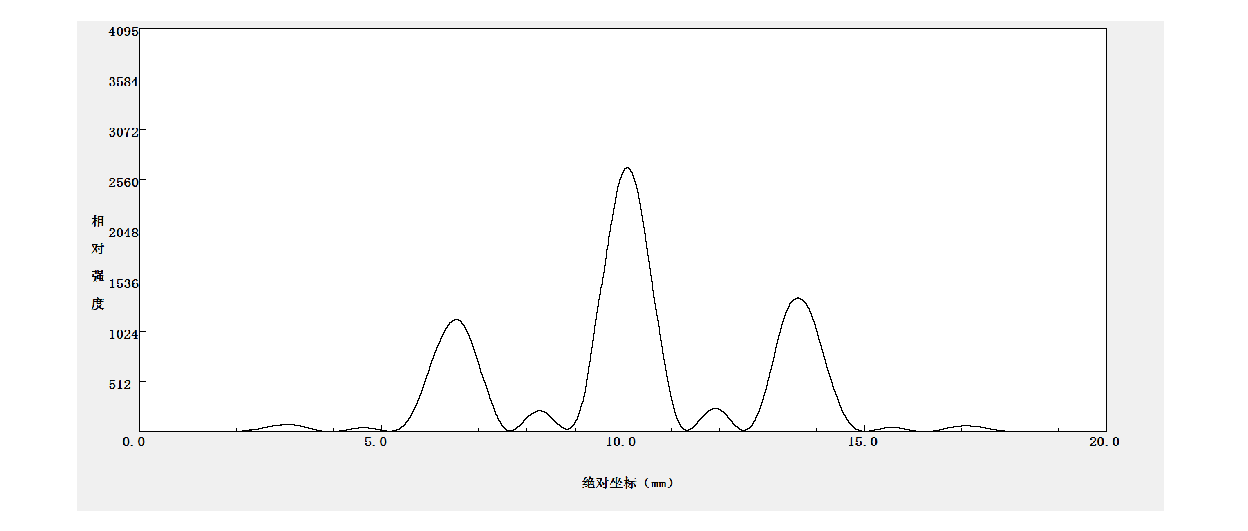
\includegraphics[width=\textwidth]{3.eps}
  \label{fig:digit}
    
\end{figure}


观察图像可知,在最外侧暗纹出现了缺级现象。


\subsubsection{计算}
利用数据处理软件,可以得到如下的数据表:
% Table generated by Excel2LaTeX from sheet '双峰'
\begin{table}[H]
  \centering
  \caption{测量数据}
    \begin{tabular}{|c|c|c|c|c|c|}\hline
    花样名   & {零级主大值} & {左方一级极大} & {右方一级极大} & {左方缺级暗纹} & {右方缺级暗纹} \\\hline
    位置$/\si{mm}$ &10.070 & 8.250 & 11.905 & 1.145 & 18.625 \\\hline
    \end{tabular}%
  \label{tab:addlabel}%
\end{table}%

 此外,需测量一些距离参数如下表:
  % Table generated by Excel2LaTeX from sheet '单缝'
\begin{table}[htbp]
  \centering
  \caption{光学元件距离}
    \begin{tabular}{|c|c|c|}\hline
    光学元件  & {探测器} & {单缝位置} \\ \hline
    位置$/\si{\centi\meter}$ & $z_0=14.88$ & $z_1=67.50$ \\\hline
    \end{tabular}%
  \label{tab:addlabel}%
\end{table}%



本实验中所用激光器为氦氖激光器,其波长$\lambda=632.8\si{nm}$。有远场条件$z>>\frac{\rho^2}{\lambda}$成立。

\paragraph{计算缝宽}

观察图中可知,缺级条纹处:$$a=\frac{\lambda}{\sin{\theta}}$$。

并由:
$$\sin{\theta}\approx \frac{\Delta x}{z}$$

代入数据计算得:

$$a=\frac{\lambda z}{\Delta x}=38.09\si{\micro \meter}$$

式中:

$$ z=|z_1-z_0|=52.62\si{\centi \meter}$$

$$ \Delta x=8.740\si{mm}$$

下计算不确定度:

仿照前问中:从计算公式出发,可看出共有三个参数,其中$\lambda$值可视为准确值(激光器产生)。从而有如下公式:

$$\frac{\sigma_a}a=\sqrt{(\frac{\sigma_x}{\Delta x})^2+(\frac{\sigma_z}z)^2}$$

又,考虑到钢尺测距的误差(尤其是测衍射装置位置时),将其允差取为$e_{zi}=1\si{\centi\meter} $,并且,将衍射光强接收器的允差视为$e_{xi}0.010\si{mm}$(即$\pm 1$个数据点)。
$$\sigma_x=\frac{e_x}{\sqrt{3}}=\frac{e_{x1}+e_{x2}}{\sqrt{3}}=0.011\si{mm}$$

$$\sigma_z=\frac{e_z}{\sqrt{3}}=\SI{0.6}{\centi\meter}$$

得$$\sigma_a=a\times\sqrt{(\frac{\sigma_x}{\Delta x})^2+(\frac{\sigma_z}z)^2}=\SI{0.42}{\micro \meter}  $$ 
$$a \pm \sigma_a=38.1\pm 0.4 \si{\micro \meter}$$

\paragraph{计算缝间隔}

依题意,当出现一级极大时,有$$d=\frac{\lambda}{\sin{\theta}}$$

且$$\sin{\theta}\approx \frac{\Delta x}{z}$$

代入数据计算得:$$d=\frac{\lambda z}{\Delta x}=91.10\si{\micro \meter}$$

式中:

$$ z=|z_1-z_0|=52.62\si{\centi \meter}$$

$$ \Delta x=3.655\si{mm}$$

下计算不确定度:

仿照前问中:从计算公式出发,可看出共有三个参数,其中$\lambda$值可视为准确值(激光器产生)。从而有如下公式:

$$\frac{\sigma_a}a=\sqrt{(\frac{\sigma_x}{\Delta x})^2+(\frac{\sigma_z}z)^2}$$

又,考虑到钢尺测距的误差(尤其是测衍射装置位置时),将其允差取为$e_{zi}=1\si{\centi\meter} $,并且,将衍射光强接收器的允差视为$e_{xi}0.010\si{mm}$(即$\pm 1$个数据点)。
$$\sigma_x=\frac{e_x}{\sqrt{3}}=\frac{e_{x1}+e_{x2}}{\sqrt{3}}=0.011\si{mm}$$

$$\sigma_z=\frac{e_{z1}-e_{z0}}{\sqrt{3}}=\SI{1.1}{\centi\meter}$$

得$$\sigma_a=a\times\sqrt{(\frac{\sigma_x}{\Delta x})^2+(\frac{\sigma_z}z)^2}=\SI{1.00}{\micro \meter}  $$ 
$$a \pm \sigma_a=91\pm 1 \si{\micro \meter}$$
\subsection{各种屏的衍射花样}

\begin{figure}  [H]
  \begin{minipage}[t]{0.5\linewidth}  
  \centering  
  \includegraphics[width=2.2in]{fang.png}  
  \caption{单方孔}  
  \label{fig:side:a}  
  \end{minipage}%  
  \begin{minipage}[t]{0.5\linewidth}  
  \centering  
  \includegraphics[width=2.2in]{fangfang.png}  
  \caption{方孔方阵}  
  \label{fig:side:b}  
  \end{minipage}  
  \end{figure}  \begin{figure}  
    \begin{minipage}[t]{0.5\linewidth}  
    \centering  
    \includegraphics[width=2.2in]{dengbian.png}  
    \caption{等边三角形}  
    \label{fig:side:a}  
    \end{minipage}%  
    \begin{minipage}[t]{0.5\linewidth}  
    \centering  
    \includegraphics[width=2.2in]{jufang.png}  
    \caption{矩形方孔}  
    \label{fig:side:b}  
    \end{minipage}  
    \end{figure}  \begin{figure}  
      \begin{minipage}[t]{0.5\linewidth}  
      \centering  
      \includegraphics[width=2.2in]{shuangyuan.png}  
      \caption{双圆孔}  
      \label{fig:side:a}  
      \end{minipage}%  
      \begin{minipage}[t]{0.5\linewidth}  
      \centering  
      \includegraphics[width=2.2in]{danyuan.png}  
      \caption{单圆孔}  
      \label{fig:side:b}  
      \end{minipage}  
      \end{figure}  \begin{figure}  
        \begin{minipage}[t]{0.5\linewidth}  
        \centering  
        \includegraphics[width=2.2in]{yuanmi.png}  
        \caption{圆孔密排}  
        \label{fig:side:a}  
        \end{minipage}%  
        \begin{minipage}[t]{0.5\linewidth}  
        \centering  
        \includegraphics[width=2.2in]{fangmi.png}  
        \caption{方孔密排}  
        \label{fig:side:b}  
        \end{minipage}  
        \end{figure}  \begin{figure}  
          \begin{minipage}[t]{0.5\linewidth}  
          \centering  
          \includegraphics[width=2.2in]{shuangfang.png}  
          \caption{双方孔}  
          \label{fig:side:a}  
          \end{minipage}%  
          \begin{minipage}[t]{0.5\linewidth}  
          \centering  
          \includegraphics[width=2.2in]{yuanfang.png}  
          \caption{圆孔方阵}  
          \label{fig:side:b}  
          \end{minipage}  
          \end{figure}  

\section{分析与讨论}
\subsection{分析不确定度}
\paragraph{答}分析不确定度的过程见计算。
\subsection{夫琅禾费衍射和衍射结构间的关系}
\paragraph{答}夫琅禾费衍射可以看作衍射结构的傅里叶变换,夫琅禾费衍射结构可以看作空间频谱分析器,夫琅禾费衍射实现了屏函数的傅里叶变换。





      \section{收获与感想}
      本次实验是本学期的第一个实验,都说万事开头难,我也是,为这学期的实验开了个不好的头。

      实验的过程中,总是出现漏测,或者是调节不到位,因此操作比他人慢了不少,又想着早点完成实验,便出现了纰漏。

      感谢老师对我的指导,在今后的实验课程学习中,我一定会巩固自己的实验技巧,同时也会认真领会实验理论,做到脑海中有清晰的物理图像。

      同时,本次实验中我也感受到先进的技术设备对实验的提高,并了解了夫琅禾费衍射与傅里叶变换的关系,为以后的实验打下基础。


\end{document} 